\chapter{Analizadores empleados en los paquetes de web scraping}
\label{cha:analizadores empleados en los paquetes de web scraping}

Este apéndice tiene como objetivo introducir aquellos aspectos más relevantes relacionados con los
analizadores, también conocidos como \emph{parsers}, empleados en el web scraping. A lo largo de esta 
sección se realizará una pequeña sinopsis de aquellas herramientas empleadas en los algoritmos de extracción 
de los paquetes definidos en la sección \ref{sec:bibliotecas de python encontradas durante el proceso de 
busqueda}.

A modo de introducción cabe destacar que un analizador sintáctico, es un programa informático que analiza
una cadena de símbolos según las reglas de una gramática formal \cite{parser-lexer}. Generalmente, los 
analizadores se componen de dos partes, por un lado, un analizador sintáctico, y por otro un analizador 
léxico. Mientras que el analizador léxico crea tokens a partir de una secuencia de caracteres de entrada, 
el analizador sintáctico convierte los tokens en otras estructuras.

\begin{figure}[tphb]
    \centering
    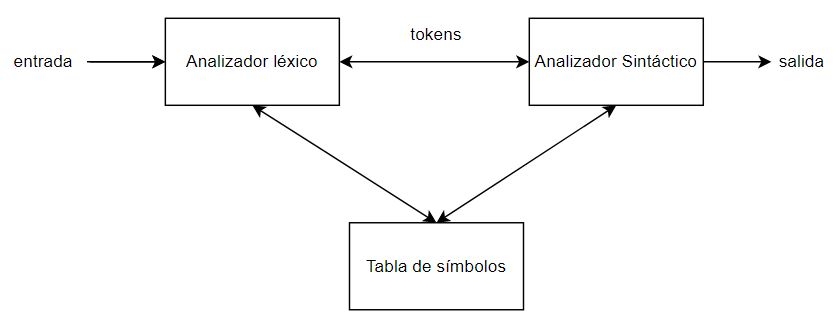
\includegraphics[width=5.5in]{parser-structure.jpg}
    \caption{Estructura basica de un analizador}
    \label{img:estructura basica de un analizador}
\end{figure}

\section{lxml}
\label{sec:lxml}

Uno de los analizadores más comunes en todos los algoritmos de minado web es \textbf{lxml} \cite{lxml}. 
Esta biblioteca de Python permite procesar tanto documentos XML como HTML.

Como la gran mayoría de analizadores, \textbf{lxml} convierte el texto de entrada en una estructura tipo 
árbol. Esto permite navegar por la propia estructura en busca de la información que se desea de forma 
sencilla. 

En el caso del web scraping, la manera en la que \textbf{lxml} es capaz de encontrar información valiosa, 
es decir texto, es a través de expresiones \emph{XPath}. Se muestra un pequeño ejemplo a continuación.

\begin{Schunk}
    \begin{Soutput}
        > html.xpath("string()")
        # TEXTTAIL

        > html.xpath("//text()")
        # ['TEXT', 'TAIL']
    \end{Soutput}
\end{Schunk}

Cabe destacar que el resultado dado por una expresión \emph{XPath} es un objeto especial que conoce parte de su
estructura. Esto permite ejecutar operaciones sobre este elemento y saber de dónde proviene a través de
diferentes métodos.

\subsection{lxml.html}
\label{subsec:lxml.html}

¿Qué ocurre con los documentos HTML mal formados? Para este propósito, se creó lo que se conoce como
\textbf{lxml.html} \cite{lxml}. Un paquete de Python especial para tratar con documentos HTML, el cual 
a diferencia del analizador base, proporciona una API de elementos propia de HTML, así como una serie de 
utilidades para tareas comunes de procesamiento de los mismos.

\begin{Schunk}
    \begin{Soutput}
        > broken_html = "<html><head><body><h1>page title</h3>"
        > parser = etree.HTMLParser()
        > tree   = etree.parse(StringIO(broken_html), parser)
        > result = etree.tostring(tree.getroot(), method="html")
        # <html><head></head><body><h1>page title</h1></body></html>
    \end{Soutput}
\end{Schunk}

Como se puede observar, incluso analizando documentos realmente mal formados, el analizador es capaz de
crear una estructura propia de un documento HTML. A partir de ahí, es posible aplicar expresiones 
\emph{XPath} con el fin de recorrer el árbol generado y recuperar información de valor.

\subsection{soupparser}
\label{subsec:soupparser}

Otro de los analizadores propios de \textbf{lxml} es \textbf{soupparser} \cite{lxml} propio del paquete
\textbf{Beautiful Soup}. La forma en la que \textbf{lxml} interactúa con \textbf{Beautiful Soup}, es a 
través del módulo \textbf{lxml.html.soupparser} el cual proporciona una seria de funciones principales. 

Por un lado, tanto \emph{fromstring()} como \emph{parse()} se emplean para analizar ya sea una cadena o un 
archivo HTML, por otro lado \emph{convert\_tree()} se emplea para convertir un árbol \textbf{Beautiful Soup} 
existente en una lista de elementos de nivel superior.

\begin{Schunk}
    \begin{Soutput}
        > tag_soup = '''<meta/><head></head><body>Hi all<p>'''
        > root = fromstring(tag_soup)
        # <html><meta/><head></head><body>Hi all<p/></body></html>
    \end{Soutput}
\end{Schunk}

Imaginemos que se dispone de una cadena HTML mal formada como la mostrada en el ejemplo. Al ser una cadena,
se emplea \emph{fromstring()} para realizar un análisis de la misma. Como vemos la salida también puede
provocar algún error, puesto que no es exactamente una estructura propia de HTML.

\section{html5lib}
\label{sec:html5lib}

\textbf{html5lib} \cite{html5lib} es un paquete de Python que implementa el algoritmo de análisis sintáctico 
de HTML5. Proporciona una interfaz similar a la del módulo \textbf{lxml.html} \ref{subsec:lxml.html} con 
métodos como \emph{fromstring()} o \emph{parse()} que operan de la misma manera que las funciones de análisis 
de HTML normales.

Al igual que \textbf{lxml.html}, este paquete también trabaja con árboles de objetos, pero en este caso 
normaliza algunos elementos y estructuras a un formato común. Por ejemplo, incluso si una tabla no tiene 
una etiqueta del tipo \emph{<tbody>}, se inyectará una automáticamente.

\begin{Schunk}
    \begin{Soutput}
        > tostring(html5parser.fromstring("<table><td>foo"))
        # '<table><tbody><tr><td>foo</td></tr></tbody></table>'
    \end{Soutput}
\end{Schunk}

\section{html.parser}
\label{sec:html.parser}

\textbf{html.parser} \cite{html-parser} es un módulo de Python que define una clase HTMLParse como base 
para analizar archivos HTML y XHTML. Este módulo trabaja alrededor de etiquetas, pues llama a métodos de 
manejo cuando se encuentran etiquetas de inicio, etiquetas finales, texto, comentarios y otros elementos 
de marcado.

\begin{Schunk}
    \begin{Soutput}
        > parser.feed('<p><a class=link href=#main>tag soup</p ></a>')
        # Start tag: p
        # Start tag: a
        # Data     : tag soup
        # End tag  : p
        # End tag  : a
    \end{Soutput}
\end{Schunk}

Como se puede observar, el algoritmo es capaz de detectar etiquetas tanto de apertura, como de cierre incluso
en documentos HTML mal formados como este. Esto hace que la búsqueda de información valiosa, en este caso
texto, sea sencilla.

\section{XML}
\label{sec:xml}

\textbf{XML} \cite{xml-cran} es un paquete de R que se encarga de realizar el análisis de documentos XML
y HTML. Además del proceso de análisis, también proporciona acceso a un intérprete de \emph{XPath} que 
permite consultar nodos concretos de los documentos. Como contrapartida, no permite el uso de selectores 
CSS para examinar XML o HTML analizados.

Adicionalmente, hay que destacar que tiene algunos problemas de liberación de memoria que no puede resolver
adecuadamente el recolector de basura de R. Por ello, se han ido creando diferentes soluciones que abordan
este problema.

En cuanto al método de análisis, se recorre el árbol buscando la información que desee y se coloca en 
diferentes formas. Hay dos maneras de hacer esta iteración. Una es "recorrer" recursivamente el árbol 
empezando por el nodo raíz y procesándolo, la otra consiste procesar cada nodo hijo de la misma manera, 
trabajando en su nombre y atributos y luego en sus hijos, y así sucesivamente.


\section{xml2}
\label{sec:xml2}

Otro paquete de R que permite trabajar con ficheros XML y HTML es \textbf{xml2} \cite{xml2-cran}. Está
basado sobre la biblioteca \textbf{libxml2}. El paquete sigue los mismos objetivos que \textbf{XML}, por
lo que el análisis de ficheros compone la parte principal del mismo.

\textbf{xml2} tiene una jerarquía de clases muy sencilla que permite no preocuparse por el tipo de objeto
se está gestionando. Estas clases son clave y se definen a continuación:

\begin{enumerate}
    \item xml\_node: un solo nodo de un documento.
    \item xml\_doc: el documento completo. Actuar sobre un documento suele ser lo mismo que actuar sobre 
    el nodo raíz del documento.
    \item xml\_nodeset: un conjunto de nodos dentro del documento. Las operaciones sobre \emph{xml\_nodesets}
    se vectorizan, aplicando la operación sobre cada nodo del conjunto.
\end{enumerate}

A diferencia del paquete \textbf{XML}, \textbf{xml2} cuida la gestión de la memoria de forma transparente,
liberando aquella que haya sido utilizada por un documento tan pronto como se pierden todas las referencias
que apuntan a él. Además, la jerarquía de clases es más simple, por lo que no es necesario pensar
exactamente qué tipo de objeto se tiene, \textbf{xml2} simplemente hará lo correcto.



